\documentclass[10pt,a4paper,twocolumn]{article}

% Ignore underfull warnings
\vbadness=10000

% Page layout
\setlength{\parindent}{.5cm}
\setlength{\columnsep}{.5cm}
\usepackage[left=2cm,right=2cm,top=2cm,bottom=2cm]{geometry}

% Encodings, characters, and typesetting
\usepackage[utf8]{inputenc}
\usepackage[T1]{fontenc}
\usepackage[english]{babel}
\usepackage{amsmath}
\usepackage{newtxtext,newtxmath}
\usepackage{microtype}

\usepackage[hidelinks,implicit=false]{hyperref}
\usepackage{orcidlink}

% Citation/reference management
\usepackage[citestyle=numeric-comp,bibstyle=numeric-comp,sorting=none,url=false,doi=false,useprefix=true,uniquename=false,uniquelist=false,giveninits=true,maxnames=2,natbib=true,backend=biber,hyperref=false]{biblatex}
\usepackage{csquotes}
\addbibresource{references.bib}
% \renewbibmacro{in:}{}
% \renewcommand{\bibopenparen}{\addcomma\addspace}
% \renewcommand{\bibcloseparen}{\addperiod}
% \DeclareFieldFormat[article,inbook,incollection,inproceedings,book,misc,unpublished]{title}{#1\isdot}
% \DeclareNameAlias{default}{family-given}
% % I have no clue why this works https://tex.stackexchange.com/a/352754
% \DeclareNameFormat{author}{%
%     \ifnumequal{\value{uniquename}}{0}
%     {\usebibmacro{name:family}
%        {\namepartfamily}
%        {\namepartgiven}
%        {\namepartprefix}
%        {\namepartsuffix}}
%     {\usebibmacro{name:family-given}
%        {\namepartfamily}
%        {\namepartgiven}
%        {\namepartprefix}
%        {\namepartsuffix}}%
%     \usebibmacro{name:andothers}}

% Use comma and space between units
\renewcommand*{\newunitpunct}{\addcomma\space}
\AtEveryBibitem{%
    \clearfield{volume}%
    \clearfield{number}%
    \clearfield{pages}%
}

% Graphics/figures/tables
\usepackage{makecell}
\usepackage{booktabs}
\usepackage{graphicx}
\usepackage{subcaption}
\graphicspath{{./figures/}}
\usepackage[font=small,labelfont=bf,labelsep=period,singlelinecheck=false]{caption}

% Leaderboard scorecard (Table~\ref{tab:leaderboard}): a TikZ dot-and-band M/P axis cell plus
% shape+luminance-distinct pass/fail glyphs (not colour, so the columns stay legible under CVD).
% Row data is generated into figures/leaderboard.tex by scripts/build_figures.py. The x-unit is
% one M/P unit; the dot radius is absolute pt so it stays circular under the stretched axis.
\usepackage{xcolor}
\usepackage{tikz}
\definecolor{prot}{HTML}{C8781F}   % warm / protective
\definecolor{alert}{HTML}{3B7DD8}  % cool / alerting
\colorlet{neutral}{black!70}
\newcommand{\pass}{\ensuremath{\bullet}}  % filled = pass
\newcommand{\fail}{\ensuremath{\circ}}    % open   = fail
\newcommand{\cmap}[1]{\raisebox{-2pt}{\includegraphics[width=2.0cm,height=0.20cm]{#1}}}
% \mprow{mean}{lo}{hi}{colour}: per-panel band (lo..hi) + mean dot on the 0..2.3 M/P axis.
\newcommand{\mprow}[4]{%
  \begin{tikzpicture}[x=1.6cm, y=1ex, baseline=-0.5ex]
    \draw[gray!25,line width=0.3pt] (0,0)--(2.3,0);
    \draw[gray!55,densely dashed,line width=0.3pt] (1,-1)--(1,1);  % white = 1
    \draw[#4,line width=2pt,line cap=round] (#2,0)--(#3,0);        % per-panel band
    \fill[#4] (#1,0) circle (1.5pt);                               % mean dot
  \end{tikzpicture}}
\newcommand{\mptick}[2]{\draw[gray!50,line width=0.3pt](#1,0)--(#1,0.5);
  \node[font=\tiny,text=gray,inner sep=1pt,anchor=south] at (#1,0.5){#2};}
\newcommand{\mpruler}{%
  \begin{tikzpicture}[x=1.6cm,y=1ex,baseline=0ex]
    \draw[gray!50,line width=0.3pt] (0,0)--(2.3,0);
    \mptick{0}{0}\mptick{1}{1}\mptick{2}{2}
    \draw[gray!55,densely dashed,line width=0.3pt](1,0)--(1,1.2);
  \end{tikzpicture}}
\newcommand{\leaderboardrows}{%
\textbf{sodium} & \cmap{strips/sodium} & \mprow{0.29}{0.24}{0.33}{prot} & 0.29 & 0.07 & \pass & \pass \\
hot & \cmap{strips/hot} & \mprow{0.44}{0.38}{0.48}{prot} & 0.44 & 0.25 & \fail & \pass\textsuperscript{*} \\
copper & \cmap{strips/copper} & \mprow{0.49}{0.46}{0.52}{prot} & 0.49 & 0.03 & \fail & \pass \\
inferno & \cmap{strips/inferno} & \mprow{0.50}{0.48}{0.52}{prot} & 0.50 & 0.45 & \pass & \pass \\
afmhot & \cmap{strips/afmhot} & \mprow{0.57}{0.52}{0.60}{prot} & 0.57 & 0.24 & \fail & \pass \\
cividis & \cmap{strips/cividis} & \mprow{0.72}{0.67}{0.74}{prot} & 0.72 & 0.44 & \pass & \pass \\
magma & \cmap{strips/magma} & \mprow{0.72}{0.72}{0.74}{prot} & 0.72 & 0.53 & \pass & \pass \\
plasma & \cmap{strips/plasma} & \mprow{0.72}{0.72}{0.75}{prot} & 0.72 & 1.02 & \pass & \pass \\
turbo & \cmap{strips/turbo} & \mprow{0.79}{0.75}{0.82}{prot} & 0.79 & 0.72 & \fail & \fail \\
viridis & \cmap{strips/viridis} & \mprow{0.83}{0.77}{0.87}{prot} & 0.83 & 0.56 & \pass & \pass \\
jet & \cmap{strips/jet} & \mprow{0.97}{0.96}{0.97}{prot} & 0.97 & 1.40 & \fail & \fail \\
\textbf{equilux} & \cmap{strips/equilux} & \mprow{1.00}{0.98}{1.01}{neutral} & 1.00 & 0.16 & \pass & \pass \\
gray & \cmap{strips/gray} & \mprow{1.00}{1.00}{1.00}{neutral} & 1.00 & 0.00 & \pass\textsuperscript{*} & \pass \\
Blues & \cmap{strips/Blues} & \mprow{1.33}{1.30}{1.37}{alert} & 1.33 & 0.40 & \pass & \pass \\
\textbf{xenon} & \cmap{strips/xenon} & \mprow{1.73}{1.67}{1.80}{alert} & 1.73 & 0.42 & \pass & \pass \\
winter & \cmap{strips/winter} & \mprow{1.76}{1.70}{1.83}{alert} & 1.76 & 1.80 & \fail & \fail \\
cool & \cmap{strips/cool} & \mprow{2.06}{1.94}{2.26}{alert} & 2.06 & 0.58 & \fail & \fail \\}
       % defines \leaderboardrows (the generated table body)
\newcommand{\leaderboardnote}{Marginal (${}^{*}$): \texttt{hot} (smallest simulated lightness step 0.001); \texttt{gray} (CAM02-UCS step CoV 0.29, PU threshold 0.30).}
  % defines \leaderboardnote (caption footnote for marginal maps)

\usepackage{siunitx}
% \unit{m/s}
% \unit{\metre\per\second}
% \unit{\frac{m}{s}}
% \sisetup{group-digits=integer,group-separator={,},group-minimum-digits={3}}
% \DeclareSIUnit[quantity-product={}]{\percent}{\%}
% % see this important post about interaction between datatools and siunitx https://tex.stackexchange.com/a/23460
% \newcommand{\meansd}[3][2]{%
%     $\num[round-mode=places,round-precision=#1]{#2} \pm %
%     \num[round-mode=places,round-precision=#1]{#3}$%
% }

% % Load data
% \usepackage{datatool}
% \DTLsettabseparator
% \DTLloaddb{totals}{../output/tables/describe-totalcounts.tsv}
% \DTLassignfirstmatch{totals}{total}{posts}{\totalposts=count}

\title{\bf A melanopic axis for scientific colormaps}
\author{
    Remington Mallett~\orcidlink{0000-0001-6183-3098} \\ % chktex 8
    Department of Psychology \\
    Northwestern University \\
    \texttt{remington.mallett@u.northwestern.edu}
}
\date{}

\begin{document}

\maketitle

\section*{Abstract}
Scientific colormaps are designed to be read: perceptually uniform, so equal data steps look equal, and robust to colour-vision deficiency (CVD).
But a colormap on a self-luminous display is also light.
Short-wavelength light drives the retinal cells (ipRGCs) that regulate the circadian system and suppress melatonin, so when a display is a viewer's dominant light source at night, as in a sleep laboratory, the spectrum a large data-fill emits is not cosmetic.
This melanopic content is standardized in lighting (CIE~S~026), but those tools take spectra as input; a colormap is a list of sRGB triples, not a spectrum, and the melanopic axis has not been applied to scientific colormaps.

We bridge that gap in four steps.
First, we define a melanopic axis for colormaps: a melanopic/photopic ratio (M/P) from three per-primary coefficients, normalized so display white --- the relevant neutral, not daylight --- equals~1, summarized per map by a mean and spread and validated via luox.
Second, treating melanopic content as a design dimension, we build Circadia, a one-parameter family of sequential colormaps, indexed by melanopic temperature ($\alpha$), that traverses the axis from protective to alerting while holding perceptual uniformity and CVD-recoverability fixed; its endpoints, Sodium and Xenon, are released.
Third, scoring colormaps in common use places them on the axis: a protective warm map already exists, popular uniform maps are melanopically smeared, and no off-the-shelf alerting map is perceptually uniform and CVD-recoverable --- the end Circadia supplies.
Fourth, we package the rater and generator as the open-source package \texttt{melanopy}.
We rate chromaticity, not dose: a colormap's physiological effect is second-order, dominated by room lighting and brightness.

\bigskip
\noindent {\bf Keywords:} \emph{colormap}, \emph{melanopic}, \emph{visual perception}, \emph{circadian}, \emph{CVD}, \emph{perceptual uniformity}, \emph{scientific visualization}

\section{Introduction}\label{sec:introduction}

Most guidance on scientific \textbf{colormaps} optimizes how a map is \emph{read}: whether equal differences in the data produce equal perceived differences in colour (\textbf{perceptual uniformity}), and whether that reading survives \textbf{colour-vision deficiency (CVD)}.
Modern map design is organized around these together with monotone ordering --- the viridis family was built to be uniform and CVD-robust~\cite{smith2015viridis}, cividis optimizes explicitly for CVD~\cite{nunez2018cividis}, Kovesi's CET maps systematize uniformity~\cite{kovesi2015colourmaps}, Moreland's diverging maps solved the midpoint problem for signed data~\cite{moreland2009diverging}, and Crameri's work documents how much colour misuse still distorts science~\cite{crameri2020colour}.
These are the right priorities for almost every figure.

\par
But a colormap is also \emph{light}.
On a self-luminous display a large data-fill --- a spectrogram, a density map, a heat map --- covers a substantial fraction of the screen and therefore emits a substantial fraction of the screen's light.
When the viewer is in a dark room and the display is their dominant light source, the \emph{spectrum} of that emitted light is not cosmetic: short wavelengths drive the intrinsically photosensitive retinal \textbf{ganglion cells} (\textbf{ipRGCs}) that regulate the \textbf{circadian} system and acutely suppress \textbf{melatonin}~\cite{lucas2014melanopsin,brown2020melanopic}.
This situation is not exotic.
Sleep laboratories, observatories, neonatal intensive-care units, overnight radiology reading rooms, and 24-hour control centres all put practitioners in front of data displays at night, deliberately in dim surroundings.
In all of these settings the colour content of the large fills can \emph{cooperate with} --- or \emph{fight} --- whatever circadian-lighting strategy the room is running.

\par
Colormap craft offers no vocabulary for this.
Where collections add organizing structure, they sort by \emph{structure} itself (Crameri), by \emph{domain} (cmocean~\cite{thyng2016cmocean}), or by \emph{data type} (\textbf{ColorBrewer}~\cite{harrower2003colorbrewer}) --- \textbf{none by circadian or melanopic content.}
Perceptual uniformity and CVD-safety are, in effect, the two axes the field already navigates; melanopic content is a further design dimension --- one the colormap-design literature has not adopted, even though energy-aware visualization has shown that a physically related (blue-dominated) display axis can drive colormap construction.
The gap we fill is a \emph{standardized melanopic} axis for scientific colormaps, with a bidirectional framing the energy-minimization view does not support.

\par
The \textbf{metrology} to fill it already exists.
Quantifying melanopic light is a solved, standardized problem: the \textbf{CIE} S 026:2018 system defines the melanopic action spectrum and the $\alpha$-opic quantities~\cite{cie_s026_2018}, formalizing the framework of Lucas et al.~\cite{lucas2014melanopsin}; melanopic equivalent daylight illuminance predicts circadian responses across a wide range of conditions~\cite{brown2020melanopic}; and validated open implementations exist (\textbf{luox}~\cite{spitschan2021luox}, LuxPy, and Colour).
Crucially, these tools take \textbf{spectral power distributions} as input.
They do not answer ``where does viridis sit?'', because a colormap is a list of \textbf{sRGB} triples, not a spectrum. % chktex 38
We build directly on this metrology rather than reinventing it; our work is the missing adapter from colormaps to the established melanopic measure.

\par
We contribute: (i) a \textbf{rater} that scores any colormap on a melanopic axis; (ii) a one-parameter \textbf{generator} that traverses the axis while holding perceptual uniformity and CVD-recoverability fixed; (iii) a \textbf{scored index} of colormaps in common use, which places them on the axis and confirms the gap the generator fills; and (iv) the open-source package \textbf{melanopy} bundling all three.
The axis and the constrained generator are the headline; the index confirms the landscape rather than motivating it.

\section{The melanopic axis}\label{sec:axis}

\paragraph{The axis as a design dimension.}
The central conceptual move is to treat melanopic content as a \textbf{design dimension, not a pass/fail rule}.
Perceptual uniformity and CVD-safety are \emph{universal requirements}: every map should clear them, and a map that fails is simply worse.
Melanopic content is different. Every map sits \emph{somewhere} on the axis, and ``good/bad'' does not apply --- only \emph{which regime suits which context}:

\begin{itemize}
    \item \textbf{protective} --- warm, low \textbf{melanopic ratio} (M/P < 1);
    \item \textbf{alerting} --- cool / blue-rich, high melanopic ratio (M/P > 1),
\end{itemize}

with \textbf{display white as the unit} (M/P = 1).
A daytime alertness display and an overnight sleep-lab display want opposite ends of the same axis; neither end is ``correct'' in the abstract.

\par
\textbf{The area-weighted melanopic budget.} Why does the axis matter for some marks and not others?
Because emitted light scales with screen area. Large fills --- spectrograms, density maps, heat maps --- cover a big fraction of the display and dominate the light it emits, so the axis matters for them.
Small categorical marks --- lines, points, glyphs --- emit negligibly regardless of their colour, so for them the axis is effectively \emph{``ignore it''}: a single CVD-safe categorical palette serves every circadian regime.
This split is a design principle, not a limitation: it tells us to spend the melanopic budget on \emph{sequential fills} and to keep categorical colour a separate, fixed concern.
(\textbf{Melanopy} ships exactly one CVD-safe categorical palette, justified by this argument; it stays well-separated under simulated colour blindness, Fig.~\ref{fig:melanopic-colormaps}.)

\begin{figure}[t]
    \centering
    
\includegraphics[width=\columnwidth]{melanopic_colormaps.png}
    \caption{The area-weighted budget in practice. \emph{Top:} the protective endpoint Sodium under simulated dichromacy stays order-preserving --- lightness does the ordering work. \emph{Middle/bottom:} the single CVD-safe categorical palette stays well-separated under colour blindness, so one palette serves every circadian regime.}\label{fig:melanopic-colormaps} % chktex 12
\end{figure}

\paragraph{The spectral half: from a spectrum to three coefficients.}
The melanopic content of light is a standardized quantity, and we adopt the standard rather than approximate it.
For a spectral power distribution $S(\lambda)$, the melanopic-to-photopic ratio is
\begin{equation}
  R(S) = \frac{\int S(\lambda)\,s_{\mathrm{mel}}(\lambda)\,\mathrm{d}\lambda}
              {\int S(\lambda)\,V(\lambda)\,\mathrm{d}\lambda},
  \label{eq:R}
\end{equation}
with $s_{\mathrm{mel}}$ the \textbf{CIE S 026:2018 melanopic action spectrum} and $V$ the \textbf{CIE 1931 $2^{\circ}$ $V(\lambda)$ photopic function}, both vendored from the source tables.
A display's fixed primaries $P_R, P_G, P_B$ reduce this to three per-primary coefficients,
\begin{equation}
  \mu_c = R(P_c), \qquad c\in\{R,G,B\},
  \label{eq:mu}
\end{equation}
the entire display-dependent part of the model.
We anchor to the standard through the melanopic daylight-efficacy ratio,
\begin{equation}
  \mathrm{mel\text{-}DER}(S) = R(S)/R(\mathrm{D65}),
  \label{eq:melder}
\end{equation}
the quantity luox reports ($\mathrm{D65}\equiv 1$).
The melanopic response peaks at \textbf{490 nm} as expected, and display gray stays pinned at \textbf{1.000} (Fig.~\ref{fig:s026-validation}).
This is the same weighting the validated luox calculator~\cite{spitschan2021luox} is built on, and we confirm our implementation against it: Melanopy's spectral engine reproduces the CIE S 026 D65 melanopic ELR normalization constant --- the quantity luox is pinned to --- to five significant figures (1.32621 vs 1.3262 mW/lm), and yields the expected melanopic daylight-efficacy ratios (mel-DER) for the standard illuminants (D65 = 1.000 by definition, equal-energy = 0.906, Illuminant A = 0.496).
Method and a luox-uploadable spectrum set are in the companion \texttt{luox-crosscheck.md}.

\begin{figure}[t]
    \centering
    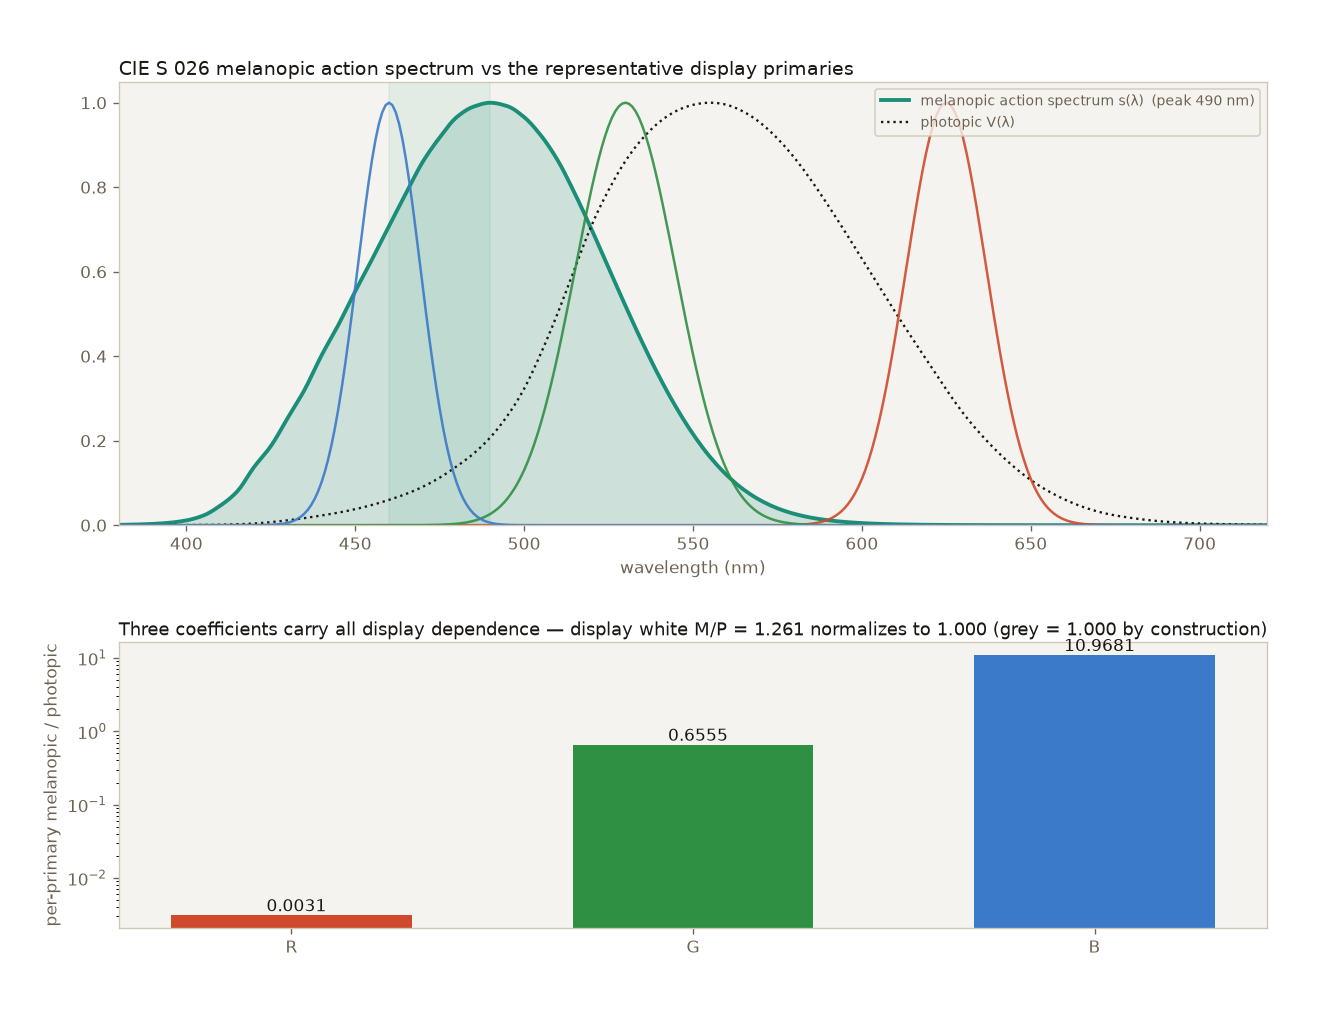
\includegraphics[width=\columnwidth]{s026_validation.png}
    \caption{CIE S 026 validation: the melanopic action spectrum (peak 490 nm), display gray pinned at 1.000, and the leaderboard ranking unchanged (every map moved $\leq 0.035$) when an earlier analytic template is replaced by the validated spectrum.}\label{fig:s026-validation}
\end{figure}

\par
For the representative panel, the three coefficients $\mu_c$ are:

\begin{center}
    \begin{tabular}{lc}
        \toprule
        primary & coefficient $\mu_c$ (M/P) \\
        \midrule
        R & 0.0031 \\
        G & 0.6555 \\
        B & 10.9681 \\
        \bottomrule
    \end{tabular}
\end{center}

The blue primary does almost all of the melanopic work --- $\mu_B \gg \mu_G \gg \mu_R$ --- which is precisely why the axis is mostly a warm $\leftrightarrow$ cool story, and why the warm/cool spread asymmetry of Section~\ref{sec:circadia} is fundamental rather than incidental.
These three numbers are regression-locked to the validated spectrum, so the data and the numbers cannot silently drift apart.

\paragraph{The colormap half: from sRGB to mean and spread.}
The rater turns a colormap into numbers on the melanopic axis.
A colour $\mathbf{c}=(r,g,b)$ in sRGB is linearized by the sRGB transfer function,
\begin{equation}
  \tilde c =
  \begin{cases}
    c/12.92, & c \le 0.04045,\\
    \bigl((c+0.055)/1.055\bigr)^{2.4}, & c > 0.04045,
  \end{cases}
  \qquad c\in\{r,g,b\},
  \label{eq:eotf}
\end{equation}
and with the exact sRGB luminance weights $w_R,w_G,w_B$ (summing to $1$),
\begin{equation}
  Y = \sum_c w_c\,\tilde c, \qquad M = \sum_c w_c\,\tilde c\,\mu_c .
  \label{eq:YM}
\end{equation}
Here $Y$ is the \textbf{photopic luminance} and $M$ its melanopic analogue, each channel weighted by the coefficient $\mu_c$ of \eqref{eq:mu}.
The melanopic ratio, normalized so display white equals $1$, is
\begin{equation}
  \mathrm{M/P}(\mathbf{c}) = \frac{1}{R_{\mathrm{white}}}\frac{M}{Y}
    = \frac{1}{R_{\mathrm{white}}}
      \frac{\sum_c w_c\,\tilde c\,\mu_c}{\sum_c w_c\,\tilde c},
  \qquad R_{\mathrm{white}} = \sum_c w_c\,\mu_c .
  \label{eq:mp}
\end{equation}
The inner factor is a luminance-weighted average of the three $\mu_c$; since $\mu_B \gg \mu_G \gg \mu_R$ the blue primary dominates.
At white ($\tilde c\equiv 1$), $M/Y = R_{\mathrm{white}}$, so $\mathrm{M/P}=1$ by construction.
The per-colour SPD $rP_R+gP_G+bP_B$ is therefore conceptual only --- the collapse to \eqref{eq:mp} means it is never formed at runtime.

\par
\textbf{Two metrics: where the map sits, and how tightly.}
A single mean would hide the structure that matters, so the rater reports \textbf{two distinct quantities}, both \textbf{luminance-weighted} (plus the raw per-position range; the full per-position profile behind both is in Appendix~\ref{app:profiles}, Fig.~\ref{fig:profiles}).
A colormap is colours $\mathbf{c}_i$ at positions $t_i\in[0,1]$, $i=1,\dots,N$, with $\rho_i=\mathrm{M/P}(\mathbf{c}_i)$ and luminance $Y_i$.
Near-black positions (which emit almost nothing) are dropped --- leaving $\mathcal{E}=\{\,i : Y_i > 0.01\,Y_{\max}\,\}$ so neither number is dominated by the dark end of the ramp --- and the two are luminance-weighted over $\mathcal{E}$:
\begin{align}
  \overline{\mathrm{M/P}}
    &= \frac{\sum_{i\in\mathcal E} Y_i\rho_i}{\sum_{i\in\mathcal E} Y_i}
    && \text{(M/P mean --- where the map sits),} \label{eq:mean}\\
  \sigma
    &= \sqrt{\frac{\sum_{i\in\mathcal E} Y_i(\rho_i-\overline{\mathrm{M/P}})^2}
                  {\sum_{i\in\mathcal E} Y_i}}
    && \text{(M/P spread --- how tightly).} \label{eq:spread}
\end{align}
The mean says \emph{where} the map sits (display white = 1; $<1$ protective, $>1$ alerting); the spread says \emph{how tightly} --- a tight $\sigma$ reads as a ``pure'' ramp.

These two are the axis's \emph{measured outputs} --- distinct from the generator's \emph{input} dial introduced in Section~\ref{sec:circadia}.
They are also independent of each other, and the gap between them is the point (all maps are plotted in this mean--spread plane in Appendix~\ref{app:mean-spread}).
viridis sits mid-axis (M/P 0.83 --- mildly protective on \emph{average}) yet has a high spread ($\sigma$ 0.56): it dumps high-melanopic blue at its dark, low-data end, so it is \emph{smeared}, not tight.
A protective mean and a pure ramp are different properties, and a map can have one without the other.
(Concretely, \texttt{rate\_colormap(viridis)} returns \texttt{melanopic\_ratio = 0.834}, \texttt{mp\_spread = 0.556}, \texttt{range = (0.395, 3.069)}.) % chktex 36

\par
\textbf{Display-panel dependence.}
Melanopic content depends on the display's primary spectra, which sRGB does \textbf{not} fix.
The rater therefore takes a \texttt{panel} argument selecting among representative archetypes --- narrowband RGB (default), blue-pump white-LED LCD, OLED, and quantum-dot wide-gamut.
Absolute M/P shifts with the panel (the blue coefficient ranges $\approx 8.8$ for OLED to $\approx 13.7$ for wide-gamut), but the \textbf{ranking is robust} to it (Section~\ref{sec:existing-colormaps}).
For exact numbers on a specific monitor, a user plugs that monitor's measured primary SPDs into \texttt{melanopy.spectra.coefficients\_from\_primaries} and obtains its own three coefficients --- swapping panels means swapping just those three numbers.

\par
Section~\ref{sec:existing-colormaps} places colormaps in common use on this axis (Table~\ref{tab:leaderboard}).

\section{The Circadia family: a uniformity-preserving generator}\label{sec:circadia}

Treating melanopic content as a design dimension --- not a fixed property --- invites a tool that traverses it: a one-parameter family that moves a colormap from protective to alerting on demand.
The difficulty, and the contribution, is that this cannot be done naively --- raising a ramp's melanopic ratio by shifting it bluer destroys the perceptual uniformity and CVD-recoverability a scientific colormap must keep.
The \textbf{Circadia family} (\texttt{mp.circadia(alpha)}) traverses the axis while holding both fixed. % chktex 36

\begin{figure}[t]
    \centering
    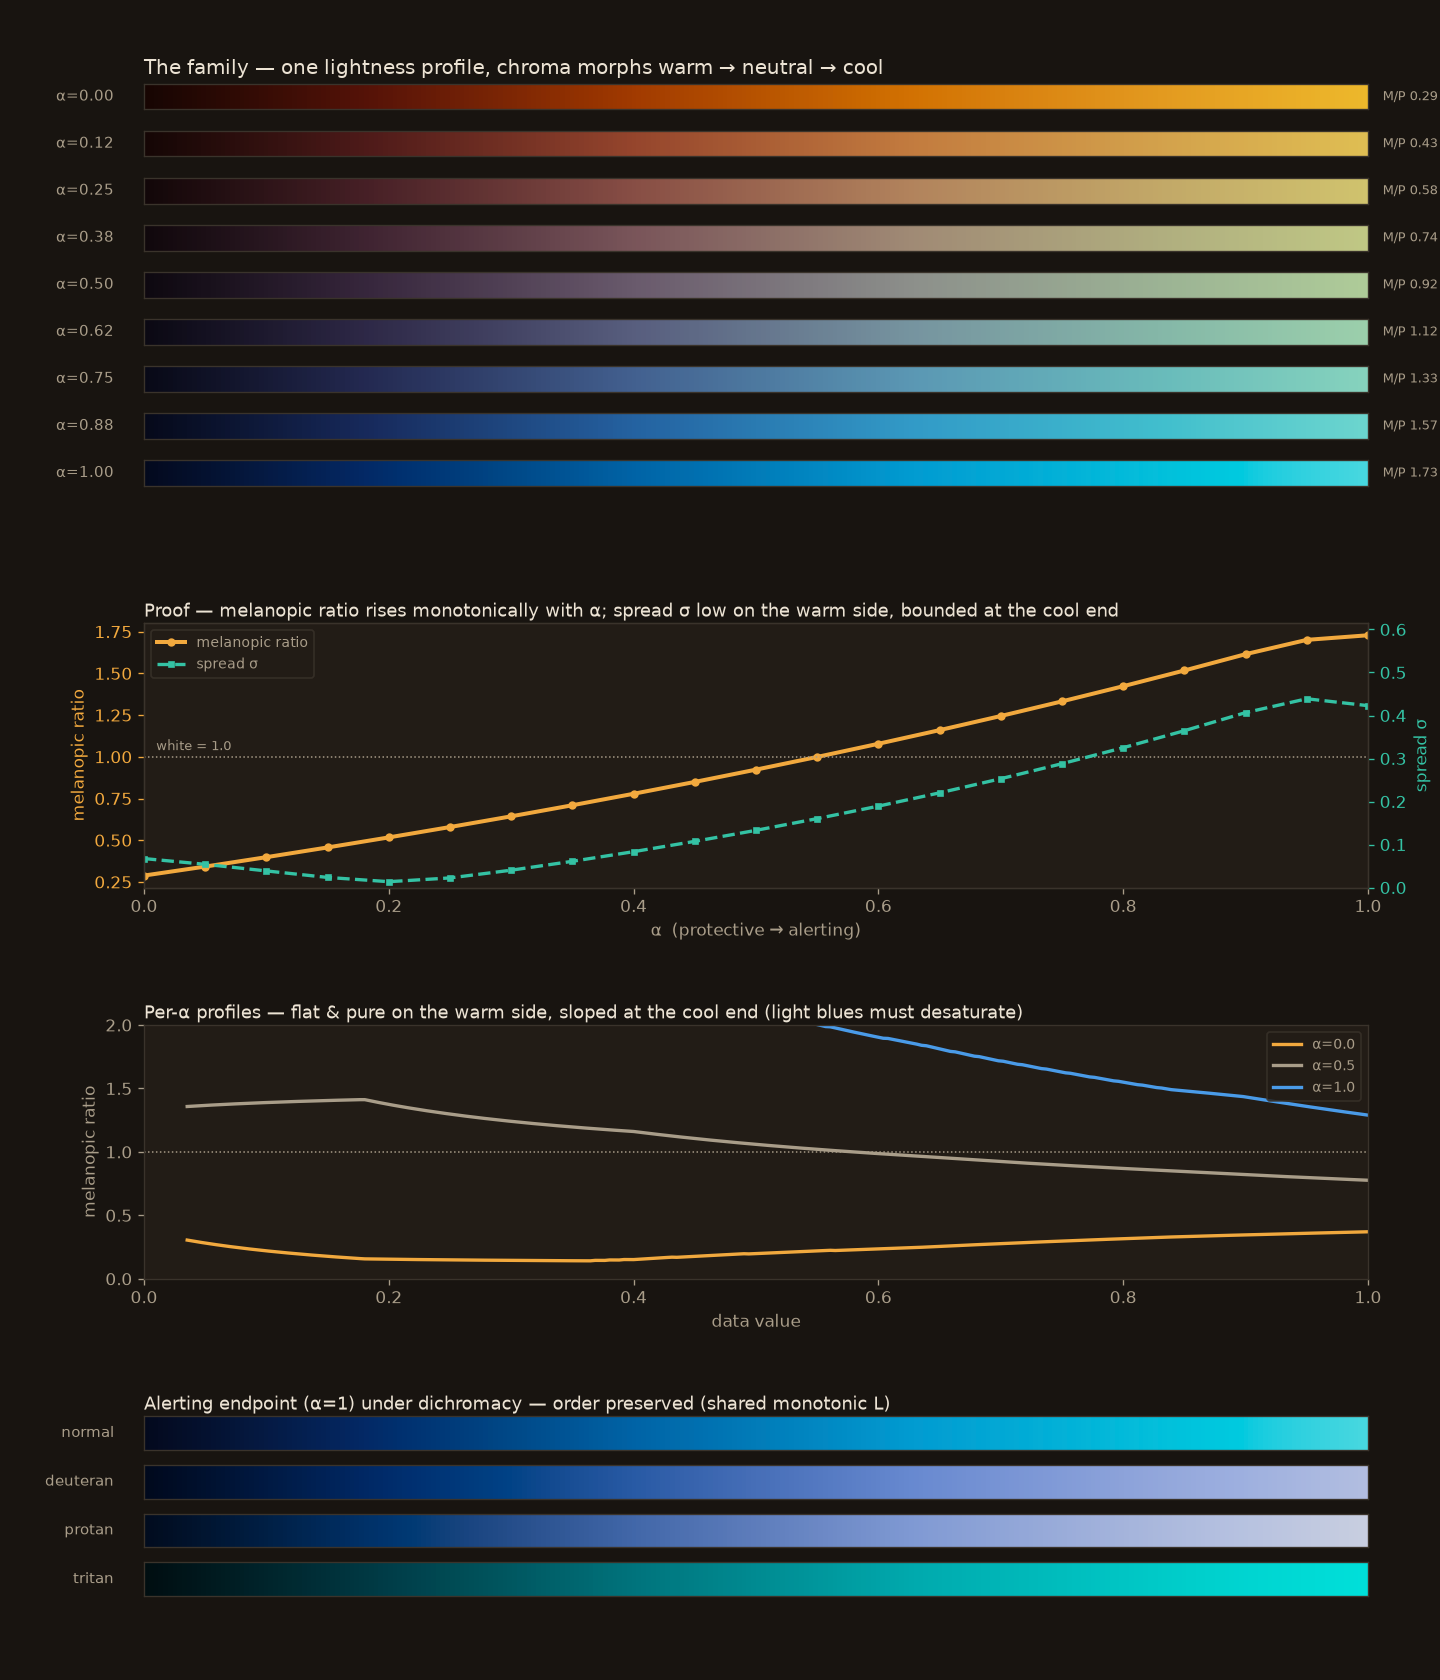
\includegraphics[width=\columnwidth]{circadian_generator.png}
    \caption{The Circadia family swept across $\alpha$ from the protective endpoint Sodium ($\alpha = 0$) through the neutral Equilux ($\alpha \approx 0.55$) to the alerting Xenon ($\alpha = 1$). Lightness rises identically for every $\alpha$; only the chroma path changes.}\label{fig:circadian-generator}
\end{figure}

\par
\textbf{The dial and the measurement are different things.}
The family's single design parameter is $\alpha \in [0, 1]$, a dimensionless dial we call the \textbf{melanopic temperature}: 0 is protective (warm), 1 is alerting (cool).
$\alpha$ is an \emph{input} --- a geometric position on an \textbf{OKLab} morph (below) --- not a melanopic measurement.
What the rater reports, the \textbf{M/P mean} and \textbf{M/P spread} of Section~\ref{sec:axis}, are \emph{outputs} measured from the rendered colours.
For the Circadia family the M/P mean is an emergent, monotone function of $\alpha$ (measured 0.29 $\rightarrow$ 1.73 on the default panel), so turning the dial does move a map along the axis --- but the two are not the same quantity.
$\alpha$ is dimensionless and panel-independent; the M/P mean is a measured optical ratio that shifts with the display.
And the M/P spread is orthogonal to $\alpha$ altogether: the dial sets \emph{where} a map sits, not \emph{how tightly}, and the warm/cool asymmetry below shows the spread is governed by the gamut, not the knob.
In short, \textbf{$\alpha$ is what you set; M/P mean and M/P spread are what you measure.}

\begin{table*}[t]
    \centering
    \caption{The Circadia anchors: the dial position $\alpha$, the measured M/P on the default panel, and the character of each.}\label{tab:anchors}
    \begin{tabular}{lccl}
        \toprule
        anchor & $\alpha$ & M/P (measured) & character \\
        \midrule
        \textbf{Sodium} & 0.00 & 0.29 & warm, protective, pure \\
        \textbf{Equilux} & 0.55 & $\approx 1.00$ & neutral (M/P = 1 crossover, true $\alpha \approx 0.5505$) \\
        \textbf{Xenon} & 1.00 & 1.73 & cool, alerting \\
        \bottomrule
    \end{tabular}
\end{table*}

The anchors carry evocative names while the measured quantities keep the precise optical term: \textbf{Sodium}, \textbf{Equilux}, and \textbf{Xenon} name points on the dial; \textbf{M/P mean} and \textbf{M/P spread} name what is measured there --- motivation for what is designed, precision for what is reported.

\par
\textbf{Why uniformity comes for free.}
The generator is pure OKLab geometry~\cite{ottosson2020oklab}; it never looks at the melanopic coefficients of Section~\ref{sec:axis}.
A \textbf{single monotone lightness profile $L(t)$}, shared by every $\alpha$, is paired with two endpoint chroma paths $\mathbf{ab}_{\mathrm{warm}}(t)$ and $\mathbf{ab}_{\mathrm{cool}}(t)$ in the OKLab $(a,b)$ plane.
For melanopic temperature $\alpha\in[0,1]$,
\begin{align}
  \mathbf{ab}(t,\alpha) &= (1-\alpha)\,\mathbf{ab}_{\mathrm{warm}}(t)
                          + \alpha\,\mathbf{ab}_{\mathrm{cool}}(t), \label{eq:morph}\\
  \mathbf{c}(t,\alpha) &= \mathrm{clamp}_{\mathrm{sRGB}}\!\bigl(
                          \mathrm{OKLab}^{-1}\!\bigl(L(t),\,\mathbf{ab}(t,\alpha)\bigr)\bigr),
                          \label{eq:gen}
\end{align}
where $\mathrm{clamp}_{\mathrm{sRGB}}$ reduces chroma at fixed $L$ and hue for colours outside the gamut.
Because $L(t)$ is independent of $\alpha$ and $\alpha$ moves only $(a,b)$, perceptual uniformity and CVD-recoverability are governed by $L(t)$ alone and hold for every $\alpha$; the melanopic ratio $\overline{\mathrm{M/P}}(\alpha)$ is emergent and monotone (measured $0.29\to 1.73$), never computed by the generator.
The axis falls out of the geometry; it is not imposed on it.

\par
\textbf{Both properties are verified, not assumed.}
The generator's structural claims are checked numerically with \texttt{colorspacious}.
For perceptual uniformity, the CAM02-UCS lightness ($J'$) is strictly increasing along each Circadia map and the CAM02-UCS step sizes are near-constant (coefficient of variation < 0.30).
For CVD, under simulated deuteranopia, protanopia, and tritanopia (Machado et al.\ model~\cite{machado2009cvd}, severity 100) the perceived lightness stays strictly monotone, so the data order remains recoverable.
We deliberately say \textbf{CVD-recoverable}, not the stronger ``CVD-safe'': a shared monotone-lightness profile guarantees recoverable \emph{order}, which is exactly what the tests show and exactly what we claim.
The melanopic span is equally robust to the spectral choice: under the validated CIE S 026 spectrum (Section~\ref{sec:axis}) the generator's range is unchanged (0.29 $\rightarrow$ 1.73) and still monotone.

\par
\textbf{A fundamental warm/cool asymmetry.}
Sodium sits far tighter on the axis than Xenon (M/P spread $\sigma$ 0.07 vs 0.42), and this is a property of the display gamut, not a tuning miss.
Short-wavelength primaries are intrinsically low-luminance, so \emph{a light, saturated blue does not exist} --- light cool colours must desaturate toward white, where M/P $\rightarrow$ 1.
A perfectly pure \emph{protective} map is therefore achievable under a shared lightness profile, but a perfectly pure \emph{alerting} one is not.
This is a statement about the intersection of the melanopic axis with the sRGB gamut, and we report it rather than hide it (Section~\ref{sec:limitations}).

\section{Existing colormaps on the axis}\label{sec:existing-colormaps}

With the axis defined (Section~\ref{sec:axis}) and the Circadia family already in hand, we place the colormaps people already use on the axis --- a validation pass, not the motivation for the generator.
We scored every map on the default panel (display white = 1) and held each to the two universal requirements, collecting both into one scorecard regenerable from the package (Table~\ref{tab:leaderboard}).

\begin{table*}[!t]
    \centering
    \setlength{\tabcolsep}{5pt}\renewcommand{\arraystretch}{1.3}
    \caption{\textbf{The melanopic leaderboard.} Every colormap in the study on the melanopic axis (display white = 1), with the two universal requirements alongside: the \emph{ramp}; the \emph{M/P axis} cell (dot = M/P mean, bar = per-panel band across the four display archetypes); the M/P mean; the spread $\sigma$; and \textbf{PU} / \textbf{CVD-rec.}\ pass/fail. PU = monotone CAM02-UCS lightness ($J'$) with step-size CoV $< 0.30$; CVD-rec.\ = perceived lightness stays monotone under simulated deuteranopia, protanopia, and tritanopia (Machado et al., severity 100) --- the same checks applied to the Circadia family in Section~\ref{sec:circadia}. $\bullet$~pass, $\circ$~fail; ${}^{*}$~marginal (within 10\% of the PU threshold, or a near-flat CVD lightness step). Filled/open glyphs are used rather than colour so the requirement columns stay legible under CVD. Rows ascend by M/P; the ranking is stable across panels (Spearman $\rho \geq 0.99$). \leaderboardnote}\label{tab:leaderboard}
    \begin{tabular}{l c c c c c c}
        \toprule
        & & \makebox[3.68cm]{\footnotesize $\leftarrow$\,protective \hfill alerting\,$\rightarrow$}
          & & & \multicolumn{2}{c}{requirements} \\
        \cmidrule(lr){6-7}
        colormap & ramp & M/P axis & M/P & $\sigma$ & PU & CVD-rec. \\
        & & \mpruler & & & & \\
        \midrule
        \leaderboardrows
        \bottomrule
    \end{tabular}
\end{table*}

The scorecard confirms three things.
A warm, pure protective map already exists in stock \textbf{matplotlib}, so the protective end needs naming and surfacing, not new design.
The popular perceptually-uniform maps --- viridis and its siblings --- are melanopically \emph{smeared}, dumping high-melanopic blue at their dark, low-data end rather than sitting tight.
And no off-the-shelf map reaches the alerting end while staying perceptually uniform and CVD-recoverable --- precisely the slot the Circadia endpoints, Sodium and Xenon, now fill.
Because the table ranks by mean alone, it understates this last point: plotting mean against spread (Appendix~\ref{app:mean-spread}) shows the Circadia anchors holding the low-spread frontier, so \textbf{Xenon} is a tighter alerting map than \texttt{cool} despite its lower mean.
The ranking is stable across the four display panels (Spearman $\rho \geq 0.99$; per-panel and spectral-robustness detail is deferred to Section~\ref{sec:reproducibility}).

\section{Discussion}\label{sec:discussion}

The axis, the generator, and the index are only useful if they change practice without overclaiming.
This section first states what Melanopy deliberately does \emph{not} assert (Section~\ref{sec:limitations}) and then, within that honest scope, sketches where the axis could change practice (Section~\ref{sec:applications}); it closes by situating the contribution against four mature literatures (Section~\ref{sec:related-work}) and showing how every result is reproducible (Section~\ref{sec:reproducibility}).

\subsection{Limitations and honest scope}\label{sec:limitations}

Melanopy's credibility \emph{is} its contribution, so the caveats are stated plainly rather than buried.
A colormap moves only one factor of the melanopic dose, schematically
\begin{equation}
  \text{melanopic dose} \;\sim\;
  \underbrace{L\,f\,\Omega\,t}_{\text{emission \& geometry}} \times
  \underbrace{(\mathrm{M/P})}_{\text{chromaticity}} +
  \underbrace{(\text{ambient})}_{\text{room light}},
  \label{eq:dose}
\end{equation}
with $L$ screen luminance, $f$ screen-fill fraction, $\Omega$ a viewing-geometry term, and $t$ exposure: a colormap moves only the chromaticity factor, while brightness, fill, and room light dominate.

\begin{itemize}
    \item \textbf{It rates chromaticity, not dose.} We report a colour property, never a light dose or an alertness effect: in \eqref{eq:dose} a colormap touches only the M/P factor.
        If the goal is genuinely to stay alert, the dominant lever is room lighting.
    \item \textbf{Display-primary dependence.} The three coefficients assume a representative panel; real white-LED-LCD, OLED, and wide-gamut displays differ, especially in blue.
        We ship several panel archetypes and let users plug in measured SPDs.
        S 026 validates the \emph{spectral weighting}; the \emph{panel model} is orthogonal and still approximate.
        Reassuringly, the ranking is robust across panels (Section~\ref{sec:existing-colormaps}).
    \item \textbf{The warm/cool spread asymmetry is fundamental.} A perfectly pure protective map is achievable; a perfectly pure alerting one is not, because light saturated blues do not exist in the gamut (Section~\ref{sec:circadia}).
        This is a property of the axis $\cap$ the display gamut, not a defect to be tuned away.
    \item \textbf{``CVD-recoverable'', not ``CVD-safe''.} A shared monotone-lightness profile makes \emph{order} recoverable under CVD; we verify that and claim exactly that, no more.
    \item \textbf{The physiological effect is second-order.} The dominant levers are screen brightness, UI background, and room light.
        Melanopy's worth is (a) measurability, (b) the tool and index, (c) surfacing the axis, and (d) a modest \emph{non-interference} claim --- letting large fills cooperate with whatever circadian strategy the room already runs.
    \item \textbf{Prior-art scope.} The novelty claim rests on a structured related-work pass across four literatures (Section~\ref{sec:related-work}), documented separately, not a full PRISMA systematic review, and acknowledges adjacent display-hardware patents that do not address colormaps.
\end{itemize}

\subsection{Potential applications}\label{sec:applications}

The melanopic axis is a design parameter, not a delivered physiological effect.
A colormap fixes only the chromaticity factor of the melanopic dose in \eqref{eq:dose}; the dose that reaches an observer's retina multiplies that chromaticity by display luminance, screen-fill, viewing geometry, and duration.
Every application below is therefore a hypothesis the Circadia family makes \emph{expressible}, not an effect it establishes: whether a deployment delivers a circadian benefit is an empirical question, downstream of the capability this paper provides --- traversing melanopic temperature $\alpha$ while holding perceptual uniformity and CVD-recoverability fixed.
Recolouring can matter only where the display is a dominant term in that product --- large, bright, close, and viewed for sustained periods --- and where the levers that normally dominate, room lighting and screen brightness, are unavailable or deliberately held fixed.
Under that condition the same family supplies two opposite interventions, selected by moving along $\alpha$ rather than by switching between unrelated colormaps: a low-$\alpha$ tail that keeps a display beneath an ambient melanopic floor, and a high-$\alpha$ tail that turns an incidental exposure into an intentional one.
Applied at the \emph{data\,$\rightarrow$\,colour} step, both preserve uniformity and CVD-recoverability by construction, unlike a global gamma/LUT warp (\textbf{f.lux}, OS Night Shift) that tints every figure on screen and, without dimming, does not reliably reduce melatonin suppression anyway~\cite{nagare2019nightshift}.

The setting that motivated \textbf{melanopy}, overnight polysomnography (PSG), exhibits both tails at once.
The recording room is kept dark for the patient, so ambient light is unavailable as a lever for either party.
The technologist monitors physiology and the patient through instrument displays and an infrared video feed rather than by direct view of the darkened room, which removes the usual objection to a bright display at night: no scotopic sensitivity is sacrificed, because none is in use.
Their monitor subtends a large fraction of the visual field at reading distance and runs for the full shift, so its emission is a non-trivial melanopic source at the technologist's own cornea --- and through the circadian nadir a deliberately high-$\alpha$ theme turns that incidental exposure into an acute alerting dose~\cite{lockley2006shortwave}, the lever the dark room otherwise denies them.
Which screen region carries the dose depends on the view: a raw montage is sparse traces on a background, so background luminance and spectrum dominate and the alerting move is a bright, blue-white background rather than the conventional dark theme; a spectrogram or density spectral array fills the field with the colormap itself, so the alerting move is a high-melanopic ramp.
This is precisely where our reference deployment, SMACC --- a PyQt6/pyqtgraph sleep- and dream-research tool --- exposes $\alpha$ as a live slider over the large-fill colormaps (spectrogram, hypnogram density, topographic maps), while categorical line and scatter views, whose emission is negligible (Section~\ref{sec:axis}), need not react.
The same room supports the protective tail pointed the other way: light emitted toward the sleeping patient is a leak to be minimised --- a geometry problem (emission onto the operator, away from the sleeper) combined with a low-$\alpha$ theme on any patient-facing surface.
This dual use within a single room is the concrete integration target for \textbf{melanopy} in downstream tooling, which we do not evaluate here.

Bedside neuromonitoring generalises the patient-facing case with higher stakes.
Colour density spectral array and amplitude-integrated EEG are colormap displays that run continuously at the bedside, beside a patient whose circadian system is already under stress and whose environment increasingly reflects cycled-lighting protocols in neonatal intensive care~\cite{morag2024cycled}.
A protective colormap keeps such a display beneath the ambient melanopic floor the protocol establishes, rather than reintroducing the short-wavelength load the room was designed to exclude.
Here the target of protection is explicitly the patient rather than the operator, and the colormap complements --- it does not replace --- control of room light and screen placement.

The alerting tail generalises to any role that must hold vigilance through the nadir in a room kept dark or dim by design, where the operator needs no dark-adapted view of an external space.
Overnight tele-neuromonitoring is the direct sibling of PSG; windowless security and network-operations centres, dispatch floors, and remote-ICU night hubs, often kept dim to control glare across many screens, share the same structure.
In these settings the display is the only alerting surface the operator controls, and the alerting direction is the physically easy one: blue-white light is at once bright and melanopically efficient, so the intervention rides the brightness--melanopic coupling rather than fighting it, at a cost measured mainly in glare and comfort.
Because the acute alerting response to short-wavelength light is rapid~\cite{lockley2006shortwave}, an alerting theme is best deployed in bursts --- a sleep-deprived operator can dose through a slump without committing to a full night of maximal short-wavelength exposure, whose phase-shifting one would rather not impose on a rotating worker.

Several further settings meet that same condition without needing individual development:
\begin{itemize}
  \item Astronomy control floors, sonar and submarine stations, and other ``rig for red'' environments, where a perceptually uniform low-melanopic red-through-amber ramp could replace crude all-red illumination and recover the ability to read magnitude rather than only presence.
  \item Self-directed use by a solo on-call engineer or night analyst who deliberately toggles their own display into the alerting tail to stay sharp.
  \item Deliberately warm, low-lit rooms already provisioned with circadian lighting, where screens are the obvious remaining leak and a protective theme keeps the display under the melanopic budget the lighting has already paid for.
  \item Shift-scheduling and rostering interfaces, where ``melanopic-aware'' means something different: colour encodes circadian burden as \emph{data} --- flagging quick returns, backward rotations, and nadir-crossing shifts --- rather than managing the display's own emission. This is semantic use of the axis, optimised for communication rather than dose.
\end{itemize}

These applications inherit every caveat of Section~\ref{sec:limitations}; two hard exclusions bound them further.
Any role that depends on dark-adapted vision of an external environment --- a ship's bridge watch, an observatory floor, a periscope station --- disqualifies the alerting tail outright, since a bright blue-white display destroys the scotopic vision the task requires; this is the constraint that drove those fields to all-red in the first place, and PSG escapes it only because its ``outside'' is an infrared feed on another screen.
Diagnostic radiology is likewise calibrated to the DICOM grayscale standard display function, so neither tail may touch the reading itself without violating its luminance requirements; there the levers remain room light and screen area.

\subsection{Related work and novelty}\label{sec:related-work}

Four mature fields border this work, and the contribution sits in the gap between them.
(1) \textbf{Melanopic metrology:} CIE S 026~\cite{cie_s026_2018} and validated calculators~\cite{spitschan2021luox} on the $\alpha$-opic framework of Lucas et al.~\cite{lucas2014melanopsin}, with melanopic EDI predicting circadian responses~\cite{brown2020melanopic} --- all operating on SPDs, not colormaps.
(2) \textbf{Colormap craft:} perceptual uniformity, ordering, and CVD-safety~\cite{smith2015viridis,nunez2018cividis,kovesi2015colourmaps,moreland2009diverging,crameri2020colour}, with collections organized by structure, domain, or data type~\cite{thyng2016cmocean,harrower2003colorbrewer} --- none by melanopic content.
(3) \textbf{Lighting-domain melanopic modulation}, where the axis idea actually lives, but for lamps and display \emph{hardware}: metameric display tuning that varies melanopic output independent of visual appearance~\cite{allen2018metamerism} (closest prior art on the \emph{melanopic} dimension --- a 5-primary VDU for melatonin/alertness experiments, \emph{not} a colormap tool), and OS night-shift filters~\cite{nagare2019nightshift}.
(4) \textbf{Energy-aware visualization}, where a non-perceptual, display-physical property is treated as a colormap-design axis: energy-saving colour-scheme design for OLED displays optimizes colormaps to reduce display power.
GreenVis~\cite{wang2012greenvis} is a multi-objective generator that produces sequential-data colormaps minimizing OLED power for a fixed perceptual-difference budget, evaluating both pre-designed and auto-generated schemes; related work extends this to volume-rendering transfer functions~\cite{chen2016volume} and image-space dimming~\cite{chen2014imagespace}.
Because OLED power is dominated by the blue subpixel, this axis is physically near-collinear with the melanopic axis --- making it the closest structural analogue to our colormap-construction artifacts, despite a different downstream concern (battery, not melatonin).

\par
Neither building block is itself novel: the melanopic axis is mature in lighting, and the generic move of treating a display-physical property as a colormap-design axis --- with a rater, an evaluation of existing schemes, and a perception-constrained generator --- has precedent in energy-aware visualization.
Our contribution is their conjunction, plus three specific extensions.
First, the axis is a \textbf{standardized physiological quantity} (CIE S 026 melanopic, anchored to mel-DER and cross-checked against luox), not a device-specific power model or a generic perceptual-difference budget.
Second, it is \textbf{bidirectional with no privileged end}: energy-aware design is monotone-minimize and has no reason to produce a high-power map, whereas our generator deliberately walks to the high-melanopic \textbf{alerting} endpoint (Xenon) --- a regime energy-aware work would never target, and which is genuinely unexplored.
Third, we hold \textbf{CVD-recoverability} as an explicit constraint along the entire axis.
We found no precedent in the colormap-design or melanopic-metrology literatures for a melanopic rater, per-position profile, scored index, or constrained generator; the closest structural prior art is GreenVis~\cite{wang2012greenvis} (the colormap-construction dimension) and Allen et al.~\cite{allen2018metamerism} (the melanopic dimension), each adjacent along one axis but not their intersection.
This is a structured related-work pass across four literatures (English-only, without a patent-database sweep); we note that the display-hardware patent space contains adjacent per-pixel melanopic and circadian colour-cast methods, none addressing colormap design.

\subsection{Availability and reproducibility}\label{sec:reproducibility}

Everything in this paper regenerates from the open-source package: the rater, the scored index (Table~\ref{tab:leaderboard}), the Circadia generator, and every figure and table are produced by \textbf{melanopy} and its build scripts.
The per-primary coefficients are regression-locked to the CIE S 026 spectrum, so the vendored action-spectrum data and the baked numbers cannot silently drift apart, and the perceptual-uniformity and CVD-recoverability claims are checked numerically in an independent colour space (CAM02-UCS via \texttt{colorspacious}) rather than asserted.
The leaderboard ranking is robust to the display panel (Spearman $\rho \geq 0.99$ across the four archetypes; the widest single-map band is the saturated \texttt{cool}, $\approx 0.32$) and to the spectral template (replacing an earlier analytic action spectrum with the validated CIE S 026 spectrum moved every map by $\leq 0.035$ and left the order intact; Fig.~\ref{fig:s026-validation}).
A luox-uploadable spectrum set and the cross-check method are in the companion \texttt{luox-crosscheck.md}; the full source is available on GitHub (see Declarations).

\appendix
\renewcommand{\thefigure}{A\arabic{figure}}  % appendix figures number A1, A2, ...
\setcounter{figure}{0}
\section{Per-position melanopic profiles}\label{app:profiles}

Table~\ref{tab:leaderboard} compresses each colormap to a melanopic mean and spread; Figure~\ref{fig:profiles} plots the full per-position profile those two numbers summarize, for every map in the leaderboard --- the M/P mean is the luminance-weighted height of the curve and $\sigma$ is its vertical spread. Reading the M/P and emission strips together separates a genuinely low-melanopic map (a dark M/P strip throughout, e.g.\ Sodium) from a \emph{smeared} one whose M/P spikes only where the ramp emits almost no light (a bright M/P strip over a dark emission strip at the dark end, e.g.\ viridis).

\begin{figure*}[t]
    \centering
    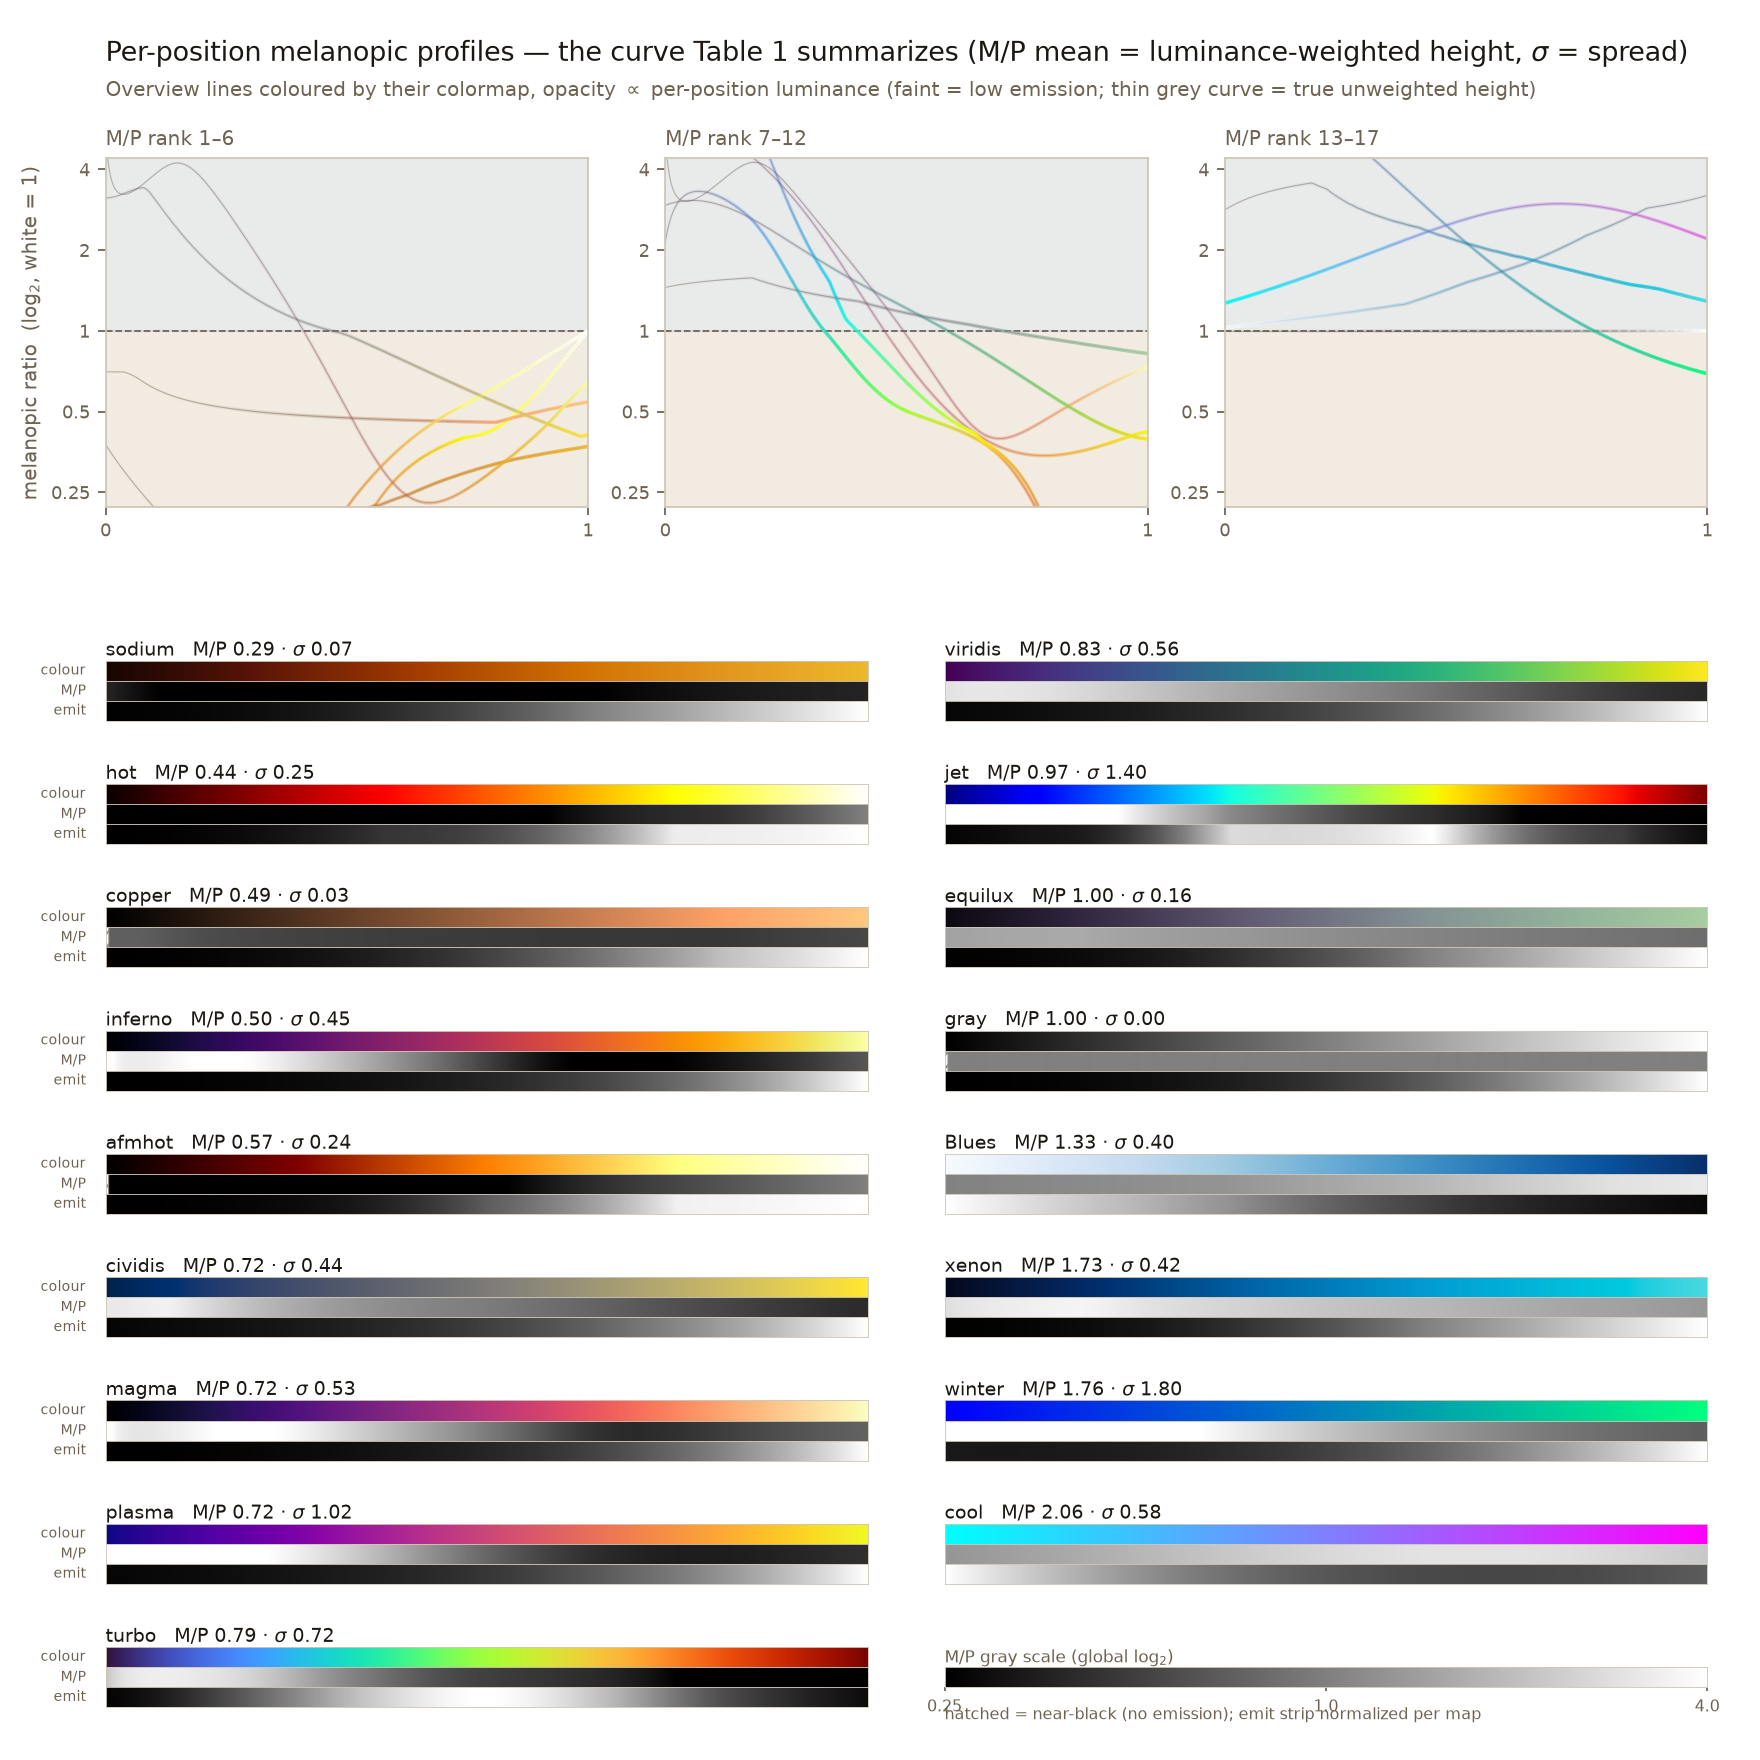
\includegraphics[width=\textwidth]{fig_melanopic_profiles.png}
    \caption{\textbf{Per-position melanopic profiles --- the profile behind Table~\ref{tab:leaderboard}.} For every colormap, the melanopic ratio at each ramp position: the un-summarized curve whose luminance-weighted height is the M/P mean and whose spread is $\sigma$ in Table~\ref{tab:leaderboard}. \emph{Top (overview):} each map's M/P curve on a shared $\log_2$ axis (white = 1, with protective/alerting shading), coloured by its own colormap with opacity tracking per-position luminance --- so a curve fades exactly where it would otherwise spike at the dark, low-emission end; a thin grey curve beneath shows the true unweighted height, and near-black positions are gaps. Maps are split into three panels by M/P rank to avoid overplotting. \emph{Below:} a triplet per map --- the \textbf{colour} ramp; the per-position \textbf{M/P} on a fixed global $\log_2$ grey scale (black = 0.25, mid-grey = 1, white = 4; near-black / no-emission positions are hatched rather than painted an extreme grey); and the per-position \textbf{emission} (photopic luminance, normalized within each map). Where the M/P strip is bright but the emission strip is dark --- e.g.\ viridis and inferno at their dark ends --- the melanopic ``spike'' carries almost no light: the honest reading of dark-end blue, and the visual form of the chromaticity-not-dose caveat.}\label{fig:profiles}
\end{figure*}

\section{The mean--spread plane}\label{app:mean-spread}
\renewcommand{\thefigure}{B\arabic{figure}}
\setcounter{figure}{0}

Table~\ref{tab:leaderboard} orders colormaps by their M/P mean alone; the spread $\sigma$ is reported alongside but does not enter the ranking. Figure~\ref{fig:mean-spread} places both on one plane --- mean on the horizontal axis (\emph{where} a map sits), spread on the vertical (\emph{how tightly} it sits there) --- so each map's position captures both at once. The Circadia anchors lie on the family's low-spread frontier: \textbf{Xenon} reaches the alerting regime ($\mathrm{M/P} > 1$) at a far smaller spread than \texttt{cool} or \texttt{winter}, which climb higher in mean only by smearing. This is the warm/cool asymmetry of Section~\ref{sec:circadia} seen across the whole index --- a tight alerting ramp and a merely high-mean one are different maps, and a ranking by mean cannot tell them apart.

\begin{figure*}[t]
    \centering
    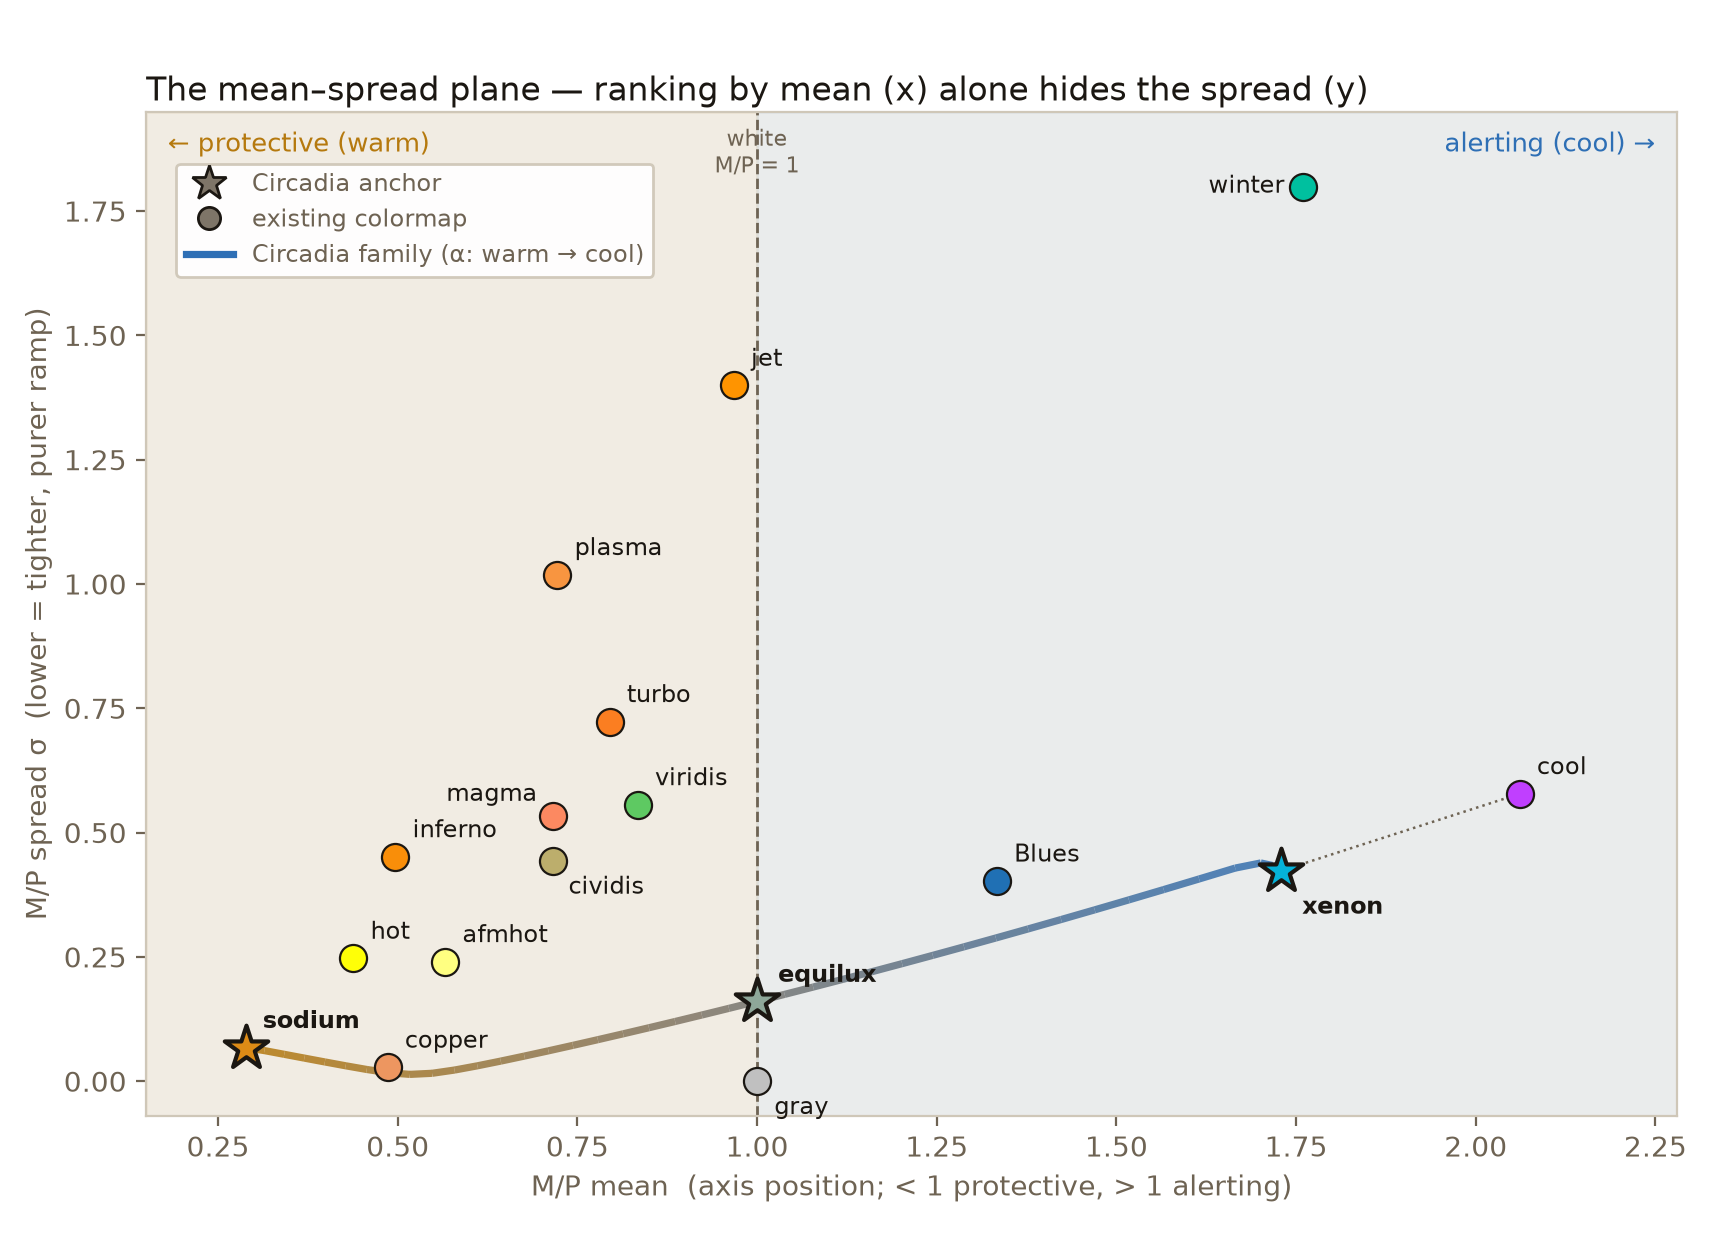
\includegraphics[width=\textwidth]{fig_mean_spread.png}
    \caption{\textbf{The mean--spread plane.} Every colormap from Table~\ref{tab:leaderboard} at its M/P mean ($x$; $<1$ protective, $>1$ alerting) and M/P spread $\sigma$ ($y$; lower is a tighter, purer ramp). Circles are existing maps coloured by their own ramp; stars are the Circadia anchors, which sit on the continuous family curve (warm $\to$ cool). The family and \texttt{copper} hold the low-spread frontier, while the popular uniform maps (viridis and siblings) and the rainbows (\texttt{jet}, \texttt{turbo}) sit high in spread. The dotted line marks the comparison in the text: \textbf{Xenon} (mean 1.73, $\sigma$ 0.42) is a tighter alerting map than \texttt{cool} (2.06, 0.58) despite a lower mean, and far tighter than \texttt{winter} (1.76, 1.80).}\label{fig:mean-spread}
\end{figure*}

\section*{Declarations}

\textbf{Availability of materials.}
All code used to generate and analyze the current corpus is publicly available on GitHub\footnote{https://github.com/remrama/melanopy}.

\smallskip
\noindent
\textbf{Acknowledgements.}
RM would like to thank Claudia Picard-Deland.

\smallskip
\noindent
\textbf{Conflict of interest.} None declared.

\section*{Glossary}

\noindent Entries in \textit{italic} are introduced in this work; those in \texttt{typewriter} denote software.

\begingroup
\renewcommand{\descriptionlabel}[1]{\hspace{\labelsep}\normalfont #1}
\begin{description}
\setlength{\itemsep}{2pt}
\item[CIE] International Commission on Illumination, the standards body behind the $V(\lambda)$, CIE 1931, and CIE S 026 definitions this work builds on.
\item[CIE 1931 $2^{\circ}$ $V(\lambda)$ photopic function] The standard photopic luminous-efficiency curve (peak near 555\,nm); the photopic term (P) of the M/P ratio.
\item[CIE S 026:2018 melanopic action spectrum] The standardized melanopsin sensitivity curve (peak near 490\,nm); the melanopic term (M) of the M/P ratio.
\item[\textit{Circadia family}] The one-parameter colormap generator introduced here, sweeping the melanopic axis (Sodium $\to$ Equilux $\to$ Xenon) at fixed perceptual uniformity and CVD-recoverability.
\item[circadian] Of the $\approx$24-hour internal clock that light entrains through ipRGC signalling.
\item[\texttt{ColorBrewer}] An online tool serving colour schemes organized by data type (sequential, diverging, qualitative).
\item[colormap] A mapping from data values to colours; the artifact this work rates and generates.
\item[CVD] Colour-vision deficiency; altered colour discrimination (deuteranopia, protanopia, tritanopia) a robust map must survive.
\item[\texttt{f.lux}] A utility that warps the whole screen's colour temperature by time of day, contrasted here with adjusting colour at the data\,$\rightarrow$\,colour step.
\item[ganglion cells] Retinal output neurons; their intrinsically photosensitive subset (ipRGCs) carries the circadian light signal.
\item[ipRGCs] Intrinsically photosensitive retinal ganglion cells; melanopsin-expressing neurons driving circadian entrainment and melatonin suppression.
\item[luminance] Photometric light per unit area weighted by human brightness sensitivity (cd\,m$^{-2}$).
\item[luminance-weighted] Averaged with each colour weighted by its linear photopic luminance, so dim, low-emission steps count less.
\item[\texttt{luox}] A validated open web platform for CIE S 026 $\alpha$-opic calculations, used to cross-check the spectral engine.
\item[\texttt{matplotlib}] The Python plotting library whose stock colormaps (viridis, copper, \ldots) appear on the leaderboard.
\item[\textit{melanopic ratio (M/P)}] A colour's melanopic-to-photopic ratio, normalized so display white $=1$; $<1$ is protective (warm), $>1$ alerting (cool).
\item[\textit{melanopic temperature}] The Circadia dial $\alpha \in [0,1]$: a dimensionless, panel-independent design \emph{input} (0 protective, 1 alerting), distinct from the measured M/P.
\item[\textit{Melanopy}] The open-source package introduced here for measuring, scoring, and generating colormaps on the melanopic axis.
\item[melatonin] The hormone signalling biological night, acutely suppressed by short-wavelength light via ipRGCs.
\item[metrology] The science of measurement; here, the standardized quantification of melanopic light ported to colormaps.
\item[OKLab] A perceptual colour space (Ottosson) whose lightness/chroma geometry keeps the generated ramps uniform.
\item[perceptual uniformity] The property that equal data steps yield equal perceived colour differences along a map.
\item[photopic luminance] Cone-mediated (daylight) luminance computed with $V(\lambda)$; the P in M/P, here from exact sRGB weights ($Y$).
\item[spectral power distributions] Radiant power versus wavelength (SPD); the input melanopic metrology consumes, here rebuilt from RGB primaries.
\item[sRGB] The standard display RGB colour space; colormaps are stored as sRGB triples and linearized before spectral weighting.
\end{description}
\endgroup

\raggedbottom
\printbibliography

\end{document}